\section{Baseline}
In \citet{p9_paper}, we presented our efforts to replicate the MOC model by \citet{cleggRecalibrationMarsScience2017}.
This effort was motivated by our desire to better understand the model and its performance, and to experiment with its components in order to determine how it could be improved.
However, as discussed in that paper, there were some differences between our replica and the original model.
These differences were caused by missing information in the original paper, and so rather than introducing our own assumptions, we designed experiments to determine the best way to replicate the model.

Initially, our replication omitted the use of the \gls{mad} for outlier removal in the data preprocessing stage, a step included in the original model.
The omission was due to the lack of information regarding its implementation within the processing pipeline.
To rectify this, we experimented with applying \gls{mad} at various stages in the pipeline.
We determined that its application post-removal of the initial five shots, and prior to masking and normalization, most closely mirrored the outcomes of the original model.

Furthermore, our replica only utilized a single dataset for the \gls{ica} phase, while the original model used all five datasets.
This difference was due to the original paper not specifying how the five datasets were used, and so we designed an experiment to determine how to use them in a way that would most closely replicate the original model.
We initially assumed that the datasets were aggregated and used as a single dataset.
This approach, however, did not align with the original model's results, likely due to the loss of information from the individual datasets.
Following this discovery, we instead used the datasets in the same way as we did in the \gls{pls1-sm} phase, which yielded results aligning more closely with the original model.

Finally, our initial replica used a random train/test split for training, in contrast to the original model's manual curation to ensure representation of extreme compositions in both sets.
This difference stemmed from the original authors' application of domain expertize in their dataset curation --- a process we could not directly replicate.
Nevertheless, we found that automatically identifying extreme compositions and ensuring that they were present in both the training and testing sets brought us closer to the original model.
We chose to pull out the $n$ largest and smallest samples by concentration range, for each oxide, and reserve them for the training set.
Then we would do a random split on the remaining dataset, such that the final train/test split would be a $80\%/20\%$ split.

With these changes, we have created a more accurate replica of the \gls{moc} model, which we will use as our baseline for the rest of this paper.
As an additional measure, we have presented these changes to one of the original authors of \citet{cleggRecalibrationMarsScience2017}, who confirmed that they were reasonable and in line with the original model's implementation.

Table \ref{tab:replica_results_rmses} shows the \gls{rmse}s of the original models and our replicas after these changes.
Figure~\ref{fig:rmse_histograms} illustrates the distribution of these \gls{rmse}s as a grouped histogram.
The results show that the \gls{rmse}s of our replicas exhibit similar tendencies to the original models.
However, in some cases, our replicas have a lower \gls{rmse} than the original models, and in others, they have a higher \gls{rmse}.
These differences are due to a number of factors.

Firstly, the original models were trained with datasets from 1600mm and 3000mm standoff distances\cite{cleggRecalibrationMarsScience2017}, while we only had access to the 1600mm dataset for our replicas.
Additionally, we automated the outlier removal for the PLS1-SM phase, unlike the original manual process.
As mentioned, the original authors manually curated their training and test sets, ensuring a broad elemental range, while we implemented an automatic process for our replicas due to lack of domain expertise.
Differences might also stem from varied implementation specifics, such as programming languages and libraries used.

\begin{table*}
\centering
\begin{tabular*}{\textwidth}{@{\extracolsep{\fill}}lllllll}
\hline
Element    & \gls{pls1-sm} (original) & PLS1-SM (replica) & \gls{ica} (original) & ICA (replica) & \gls{moc} (original) & \gls{moc} (replica) \\
\hline
\ce{SiO2}  & 4.33                     & 4.52              & 8.31                 & 8.66          & 5.30                 & 5.64                \\
\ce{TiO2}  & 0.94                     & 0.50              & 1.44                 & 0.54          & 1.03                 & 0.48                \\
\ce{Al2O3} & 2.85                     & 1.80              & 4.77                 & 3.37          & 3.47                 & 1.84                \\
\ce{FeO_T} & 2.01                     & 1.94              & 5.17                 & 2.87          & 2.31                 & 1.82                \\
\ce{MgO}   & 1.06                     & 0.91              & 4.08                 & 3.01          & 2.21                 & 1.56                \\
\ce{CaO}   & 2.65                     & 1.77              & 3.07                 & 3.28          & 2.72                 & 2.09                \\
\ce{Na2O}  & 0.62                     & 0.82              & 2.29                 & 2.11          & 0.62                 & 1.34                \\
\ce{K2O}   & 0.72                     & 0.73              & 0.98                 & 1.37          & 0.82                 & 1.16                \\
\hline
\end{tabular*}
\caption{\gls{rmse}s of the original and our replicas of the \gls{pls1-sm}, \gls{ica}, and \gls{moc} models.}
\label{tab:replica_results_rmses}
\end{table*}

\begin{figure*}[ht]
	\centering
	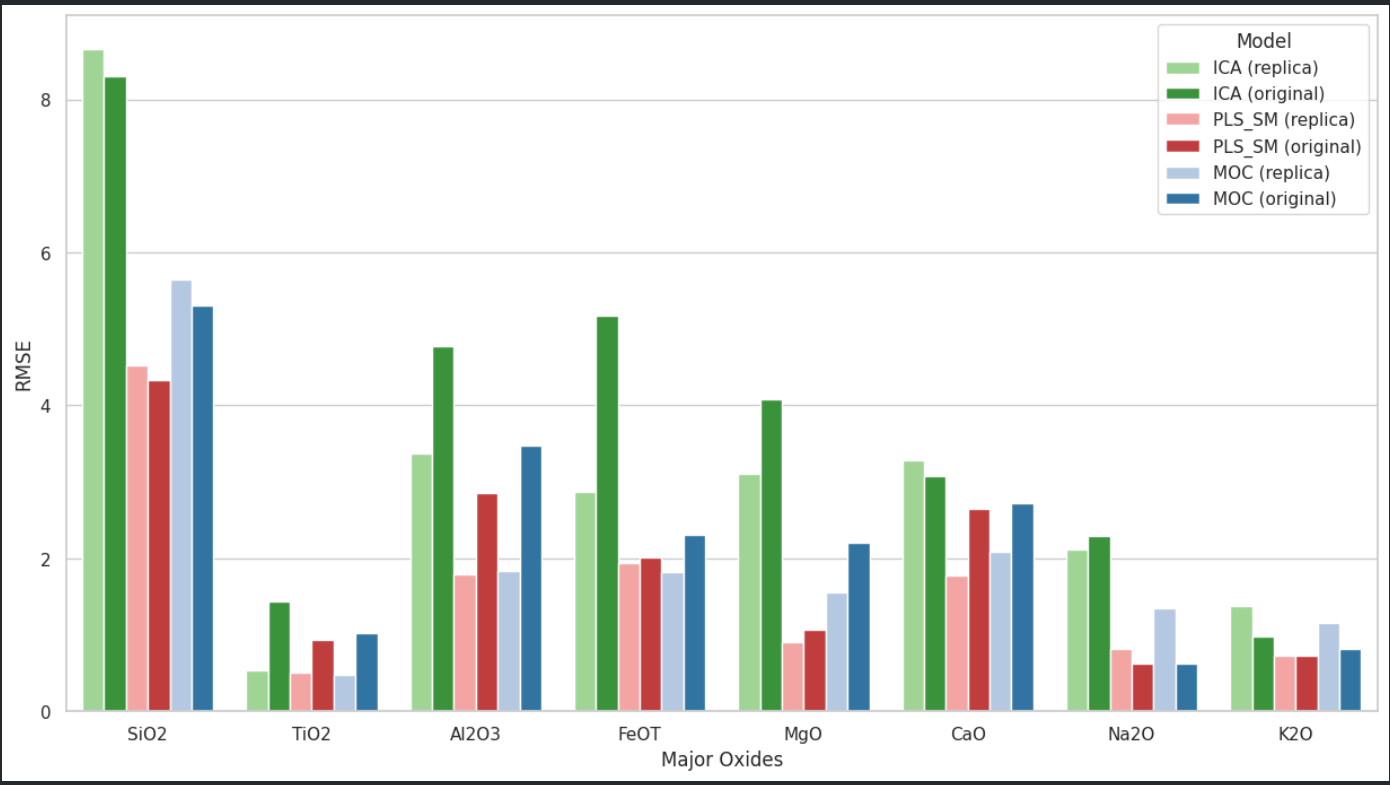
\includegraphics[width=0.85\textwidth]{images/rmse_historgram.png}
	\caption{Grouped histogram of the \gls{rmse}s of the original and our replicas of the \gls{pls1-sm}, \gls{ica}, and \gls{moc} models.}
	\label{fig:rmse_histograms}
\end{figure*}